\documentclass{article}
% Pakker for dansk sprog og font
\usepackage[utf8]{inputenc}
\usepackage[T1]{fontenc}
\usepackage[danish]{babel} 
% Pakke for at inkludere billeder
\usepackage{graphicx} 
% Pakke for matematiske symboler
\usepackage{amsmath} 
% Juster sidebredden/marginer for at få plads til to sider
\usepackage[margin=1in]{geometry} 

\title{Regressionsanalyse og Klassifikation af Bil-data: Forudsigelse af Brændstofeffektivitet}
\author{Dit Navn}
\date{\today} 

\begin{document}
\maketitle

% -----SELVE TEKSEN STARTER HER-----

\section*{Abstract}
Denne artikel præsenterer resultaterne af regressions- og logistisk regressionsanalyse lavet på biler fra datasættet 'cars.csv'. 
Målet var at forudsige brændstofeffektivitet (MPG) og klassificere biler som værende højeffektiv ved brug af finjusterede maskinlæringsmodeller (Ridge, Lasso og Logistisk Regression). 
Resultaterne viser at de finjusterede modeller præsterer robust, især den logistiske regressionsmodel demonstrerer god diskriminationsevne med AUC på 0.95.

\section{Introduktion og Problemformulering}

Formålet med denne analyse er at undersøge, hvor præcist bilers brændstofforbrug kan forudsiges og klassificeres baseret på tre nøglefeatures: vægt, hestekræfter og cylinderantal. 
Analysen er opdelt i to hovedproblemer, som skal besvares:

\begin{enumerate}
    \item \textbf{Regressionsproblem:} Hvor præcist kan vi forudsige bilens kontinuerlige brændstofeffektivitet (MPG) ved hjælp af lineære og regulariserede regressionsmodeller (Ridge og Lasso)?
    \item \textbf{Klassifikationsproblem:} Hvor pålideligt kan biler klassificeres som havende 'høj' eller 'lav' effektivitet (baseret på median MPG) ved brug af logistisk regression?
\end{enumerate}

\section{Metode}

Datasættet \texttt{cars.csv} blev indhentet. Data blev renset for manglende værdier (markeret som '?'), og features \texttt{weight}, \texttt{horsepower} og \texttt{cylinders} blev valgt som prediktorer. Data blev opdelt i et træningssæt og et testsæt (80/20 split) én gang for begge problemtyper. Alle modeller blev trænet ved brug af Scikit-learn, og finjustering blev udført ved hjælp af \texttt{Pipeline} i kombination med \texttt{GridSearchCV} og krydsvalidering for at sikre robuste resultater.

\section{Resultater og Diskussion}

Herunder vises resultaterne fra de finjusterede modeller for at besvare problemformuleringerne.

\subsection{Regressionsanalyse (MPG Prediction)}

Den indledende Lineære Regressionsmodel leverede en $R^2$ score på \textbf{0.817} på testsættet. 
Ved at anvende \texttt{RidgeCV} og \texttt{LassoCV} blev de optimale regulariseringsparametre (\(\alpha\)) fundet, for at maksimere ydeevnen og minimere overfitting.

De finjusterede Ridge- og Lasso-modeller leverede stort set identiske resultater på testsættet, med en $R^2$ score (ca. 0.817) tæt på baselinemodellen. 
Dette indikerer, at den oprindelige lineære regressionsmodel allerede var meget stabil, og at yderligere regularisering ikke var nødvendig for at forbedre den prædiktive præcision. 
Fig. 1 illustrerer, at forudsigelserne fra både Ridge og Lasso ligger meget tæt på den ideelle diagonale linje, hvilket bekræfter modellernes stærke forudsigende evne.

% --- Visualisering 1: Ridge vs Lasso ---
\begin{figure}[h]
    \centering
    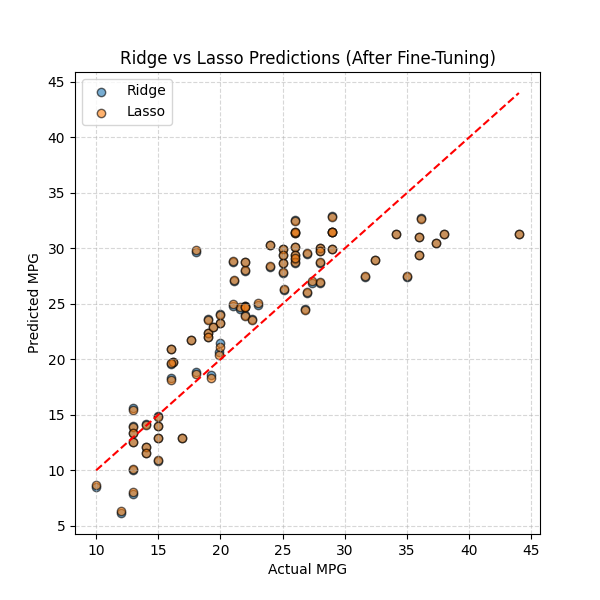
\includegraphics[width=0.75\columnwidth]{../models/ridge_vs_lasso_after_finetuning.png}
    \caption{Sammenligning af forudsigelser mellem Ridge og Lasso efter finjustering. De fleste datapunkter ligger tæt på den stiplede linje, hvilket indikerer høj præcision i forudsigelsen af MPG.}
    \label{fig:regression}
\end{figure}

\subsection{Klassifikationsanalyse (High Efficiency Prediction)}

Logistisk regressionblev brugt til at klassificere biler som værende 'højeffektiv' (\(mpg > median\)). Efter finjusteringen af parameteren \(C\) via \texttt{LogisticRegressionCV} viste modellen gode diskriminationsevner.

\textbf{Pålidelighed (AUC):} Modellen opnåede en AUC (Area Under the Curve) på \textbf{0.95} på test:

% --- Visualisering 2: ROC Kurve ---
\begin{figure}[h]
    \centering
    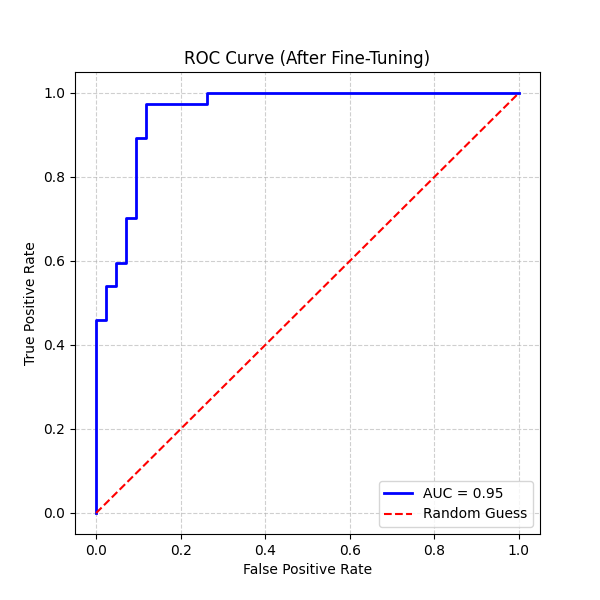
\includegraphics[width=0.7\columnwidth]{../models/roc_curve_after_finetuning.png}
    \caption{ROC-kurve for den finjusterede logistiske regressionsmodel, som viser en AUC på 0.95. Linjen ligger langt over den tilfældige gættelinje (Random Guess).}
    \label{fig:roc}
\end{figure}

\textbf{Præcision (Forvirringsmatrix):} Forvirringsmatricen (Fig. 3) bekræfter modellens præcise klassifikation. Ud af 79 observationer i testsættet:
\begin{itemize}
    \item 36 biler med lav effektivitet blev korrekt klassificeret (True Negatives, TN).
    \item 36 biler med høj effektivitet blev korrekt klassificeret (True Positives, TP).
    \item Kun 1 bil blev fejlklassificeret som 'høj', selvom den var 'lav' (False Positive, FP).
    \item 6 biler blev fejlklassificeret som 'lav', selvom de var 'høj' (False Negatives, FN).
\end{itemize}
Dette resulterer i en meget høj \textit{accuracy}, hvilket besvarer, at modellen er yderst pålidelig.

% --- Visualisering 3: Confusion Matrix ---
\begin{figure}[h]
    \centering
    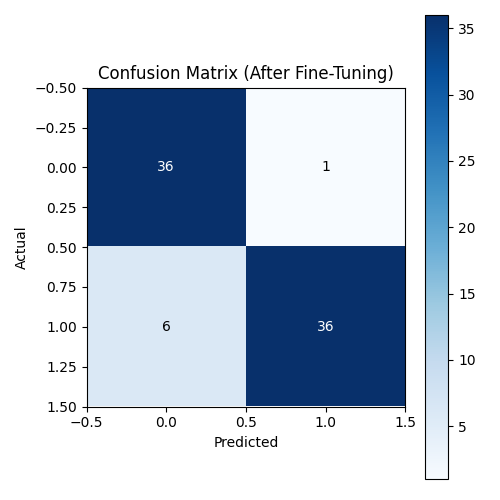
\includegraphics[width=0.6\columnwidth]{../models/confusion_matrix_after_finetuning.png}
    \caption{Forvirringsmatrix for den finjusterede logistiske regressionsmodel. Matricen viser 36 korrekte klassifikationer i hver klasse, hvilket bekræfter pålidelig prædiktion.}
    \label{fig:cm}
\end{figure}

\section{Konklusion}

Vi har opnået og finjusteret modeller for både regressions- og klassifikationsproblemer. Regressionsmodellerne (Ridge og Lasso) forudsiger MPG med høj nøjagtighed ($R^2 \approx 0.817$), hvilket indikerer et stærkt lineært forhold mellem de valgte features og brændstofeffektiviteten. Den finjusterede logistiske regressionsmodel er \textbf{yderst pålidelig} og effektiv til binær klassifikation af bilers effektivitet, bekræftet af en AUC på 0.95 og en minimal fejlrate observeret i forvirringsmatricen.

\bibliographystyle{plain}
\bibliography{references}
Scikit-learn dokumentation: \texttt{https://scikit-learn.org/stable/documentation.html}
Fag materiale af Henrik Strøm

\end{document}